\documentclass[12pt, twoside]{article}
\usepackage[letterpaper, margin=1in, headsep=0.5in]{geometry}
\usepackage[english]{babel}
\usepackage[utf8]{inputenc}
\usepackage{amsmath}
\usepackage{amsfonts}
\usepackage{amssymb}
\usepackage{tikz}
\usepackage{yhmath} %supports arc overlines
%\usetikzlibrary{quotes, angles}

\usepackage{graphicx}
\usepackage{enumitem}
\usepackage{multicol}

\usepackage{fancyhdr}
\pagestyle{fancy}
\fancyhf{}
\renewcommand{\headrulewidth}{0pt} % disable the underline of the header

\fancyhead[RE]{\thepage}
\fancyhead[RO]{\thepage \\ Name: \hspace{3cm}}
\fancyhead[L]{BECA / Dr. Huson / 10th Grade Geometry\\* 18 April 2019}

\begin{document}
\subsubsection*{10-4 Test: Volumes, circles, similar triangles, dilation ratios, transformations}
You may leave your results in terms of $\pi$ or a decimal.

 \begin{enumerate}

      \item Find the volume of a rectangular prism (box) that is 3.2 units long, 1.8 units wide, and 2.5 units high. \vspace{1.5cm}
      \item Find the area of a circle with diameter of 8. \vspace{1.5cm}
      \item Find the volume of a sphere with a radius of 14 cm. \vspace{1.5cm}
      \item Find the volume of a cone with radius 11 and a height of 18. \vspace{1.5cm}

      \item Circle $O$ has a radius $AO=6$, as shown below, and arc measure $m \wideparen{AB}=75^\circ$.
            \begin{center}
            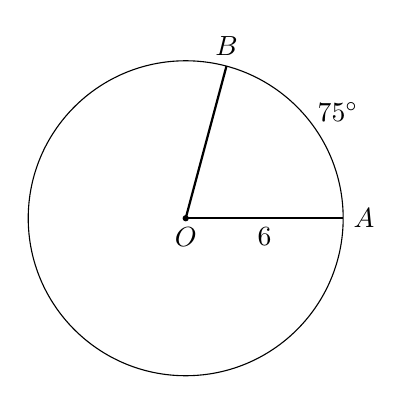
\begin{tikzpicture}[scale=.4]
              \draw (0,0) circle[radius=5];
              \draw [thick]
              (0:5) node[right] {$A$}--(0,0);
              \draw [thick] (0,0)--(75:5) node[above] {$B$};
              \fill (0,0) circle[radius=0.1] node[below]{$O$};
              \draw (35:5.9) node{$75^\circ$};
              \draw (0:2.5) node[below]{$6$};
              %\draw (75:1.8) node[above] {$C$};
              %\draw (290:5) node[below] {$D$};
            \end{tikzpicture}
          \end{center}
          \begin{enumerate}
            \item Find the $m \angle AOB$. \vspace{1.5cm}
            \item Find the length of the arc $\wideparen{AB}$. \vspace{1.5cm}
            \item Find the area of the sector $AOB$. %\vspace{2.5cm}
          \end{enumerate}
\newpage

  \item After a dilation with center $P(1,2)$, the image of $\overline{RS}$ is $\overline{R'S'}$. If $RS=6$ and $R'S'=15$, find the scale factor of this dilation. \vspace{3cm}


  \item In the diagram below, $\triangle ABC$, with sides of 10, $x+6$, and 12, is mapped onto $\triangle DEF$ after a clockwise rotation of $90^\circ$ about point $P$.
      \begin{center}
        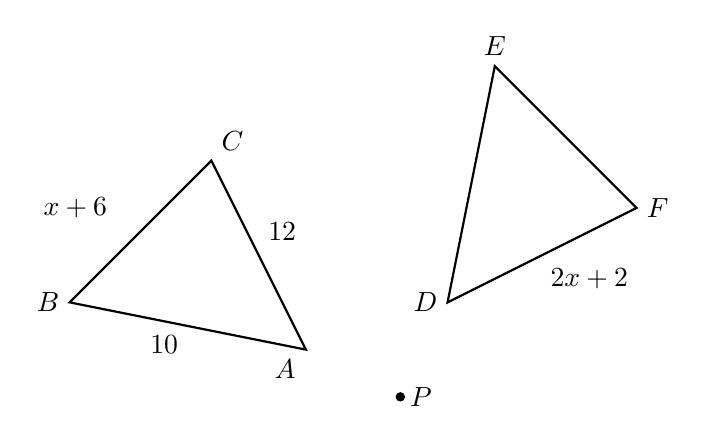
\begin{tikzpicture}[scale=.6]
        \fill (0,0) circle[radius=0.1] node[right]{$P$};
          \draw [thick]
          (-2,1) node[below left] {$A$}--
          (-7,2) node[left] {$B$}--
          (-4,5) node[above right] {$C$}--cycle;
            \node at (-5,1.5)[below]{10};
            \node at (-6,4)[left]{$x+6$};
            \node at (-2.5,3.5){12};
            \node at (4,2.5){$2x+2$};
          \draw [thick]
          (1,2) node[left] {$D$}--
          (2,7) node[above] {$E$}--
          (5,4) node[right] {$F$}--cycle;
        \end{tikzpicture}
      \end{center}
    If $DF=2x+2$, what is the value of $x$? \vspace{3cm}


     \item How many degrees is the smallest rotation around its center that would map the pentagon onto itself?
       \begin{center}
           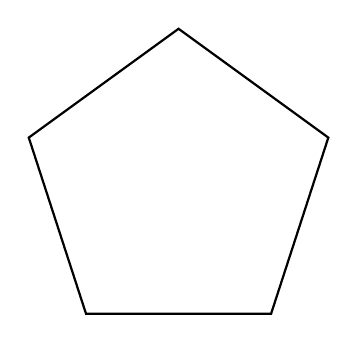
\begin{tikzpicture}%[scale=.48]
             \draw [thick]
             (18:2)--%  node[right] {$A$}--
             (90:2)--%  node[above right] {$B$}--
             (162:2)--%  node[above left] {$C$} --
             (234:2)--%  node[left] {$D$}--
             (306:2)--cycle;% node[right] {$F$}--cycle;
           \end{tikzpicture}
         \end{center}

\newpage
    \item The vertices of $\triangle JKL$ have the coordinates $J(-4,-2)$, $K(3,-1)$, and $L(-1,4)$, and the point $P(-1,2)$ is marked, as shown. \\[0.25cm]
      Apply a dilation to $\triangle JKL \rightarrow \triangle J'K'L'$, centered at $P$ and with a scale factor $k=2$. Draw the image $\triangle J'K'L'$ on the set of axes below, labeling the vertices.
      \begin{center}
        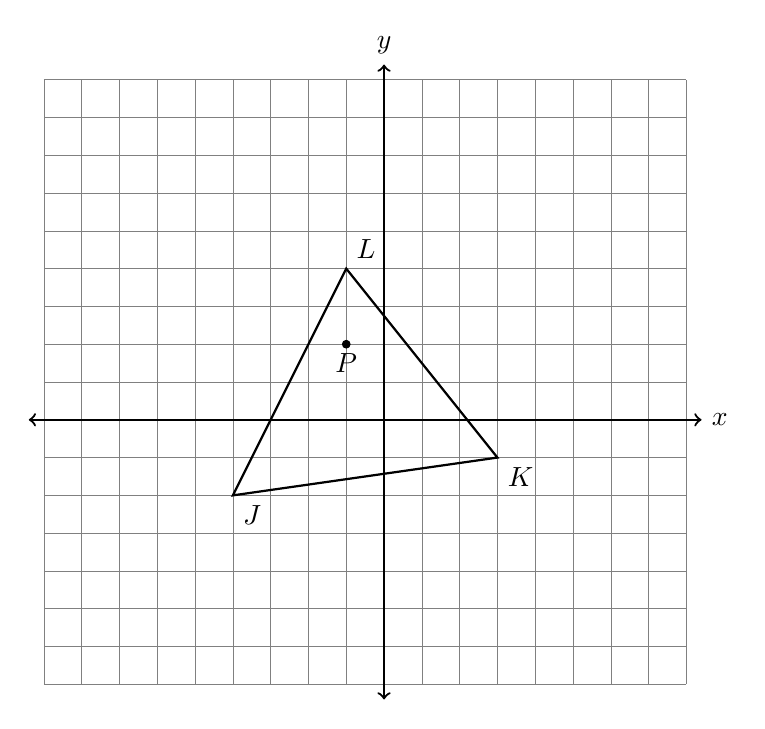
\begin{tikzpicture}[scale=.48]
          \draw [help lines] (-9,-7) grid (8,9);
          \draw [thick, <->] (-9.4,0) -- (8.4,0) node [right] {$x$};
          \draw [thick, <->] (0,-7.4)--(0,9.4) node [above] {$y$};
          \draw [thick]
          (-4,-2) node[below right] {$J$}--
          (3,-1) node[below right] {$K$}--
          (-1,4) node[above right] {$L$}--
          cycle;
          \draw [fill] (-1,2) circle[radius=0.1cm] node[below]{$P$};
        \end{tikzpicture}
      \end{center}

\item Given circle $P$ with $m \angle APB=68^\circ$.
  \begin{multicols}{2}
   \raggedcolumns
   \begin{enumerate}
     \item Write down the $m \wideparen{AB}$. \vspace{1.7cm}
     \item Find the $m\angle AQB$. \vspace{2cm}
   \end{enumerate}
     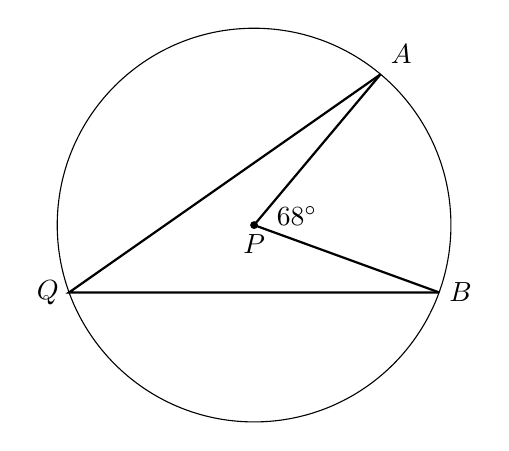
\begin{tikzpicture}[scale=.5]
       \draw (0,0) circle[radius=5];
       \draw [thick]
       (-20:5) node[right] {$B$}--
       (0,0) --
       (50:5) node[above right] {$A$};
       \draw [thick] (-20:5)--(200:5) node[left] {$Q$}--(50:5);
       \draw (35:0.4) node[right]{$68^\circ$};
       \fill (0,0) circle[radius=0.1] node[below]{$P$};
     \end{tikzpicture}
  \end{multicols} \vspace{0.5cm}

  \item Write down the center and radius of each circle. Leave radii as simplified radicals if necessary (not decimals).
    \begin{enumerate}
      \begin{multicols}{2}
      \item   $x^2+(y+1)^2=32$
      \item   $(x-1)^2+(y-3)^2=7^2$
      \end{multicols}
    \end{enumerate}

\newpage

  \item Given circle $O$ with chords $\overline{AD}$ and $\overline{BE}$ intersecting at $C$, as shown in the diagram. Given $m \wideparen{AB}=92^\circ$, $m \wideparen{BD}=88^\circ$, and $m \wideparen{DE}=70^\circ$.
    \begin{multicols}{2}
     \raggedcolumns
     \begin{enumerate}
       \item Find the $m\angle ACB$. \vspace{3.5cm}
       \item Find the measure of the minor arc, $m\wideparen{AE}$. \vspace{2cm}
     \end{enumerate}
     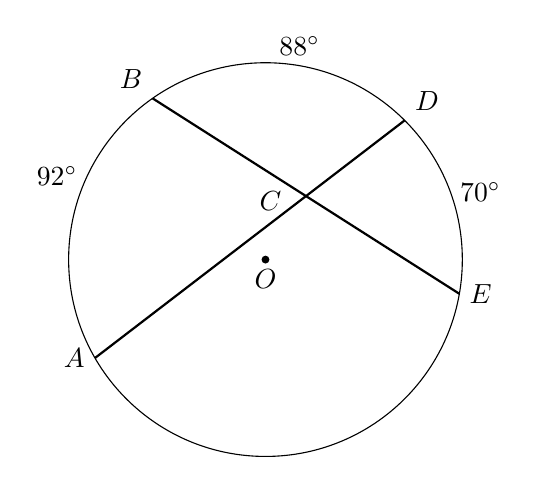
\begin{tikzpicture}[scale=.5]
       \draw (0,0) circle[radius=5];
       \draw [thick]
       (-10:5) node[right] {$E$}--
       (125:5) node[above left] {$B$};
       \draw [thick] (210:5) node[left] {$A$}--
       (45:5) node[above right] {$D$};
       \draw (85:1.5) node{$C$};
       \draw (20:5) node[right] {$70^\circ$};
       \draw (80:5) node[above] {$88^\circ$};
       \draw (155:5) node[left] {$92^\circ$};
      \fill (0,0) circle[radius=0.1] node[below]{$O$};
     \end{tikzpicture}
   \end{multicols}  \vspace{1cm}

\item The secants $\overline{ABC}$ and $\overline{ADE}$ intersect the circle $O$, as shown in the diagram. \\Given $m \wideparen{BD}=34^\circ$ and $m \wideparen{CE}=150^\circ$. Find the $m\angle A$.
     \begin{center}
     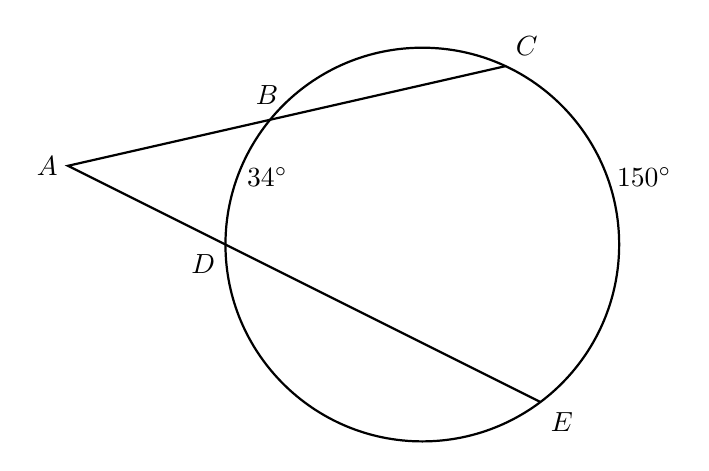
\begin{tikzpicture}[scale=.5]
       \draw [thick] (0,0) circle[radius=5];
       \draw [thick]
       (3,-4) node[below right] {$E$}--
       (-5,0) node[below left] {$D$}--
       (-9,2) node[left] {$A$}--
       (65:5) node[above right] {$C$};
       \draw (132:5.1) node[left] {$B$};
       \draw (20:5) node[right] {$150^\circ$};
       \draw (160:5) node[right] {$34^\circ$};
     \end{tikzpicture}
   \end{center} %\vspace{1cm}

    \item The secants $\overline{PQR}$ and $\overline{PST}$ intersect the circle $O$, as shown in the diagram. \\Given $m \angle P=45^\circ$ and $m \wideparen{RT}=145^\circ$. Find the $m\wideparen{QS}$.
         \begin{center}
         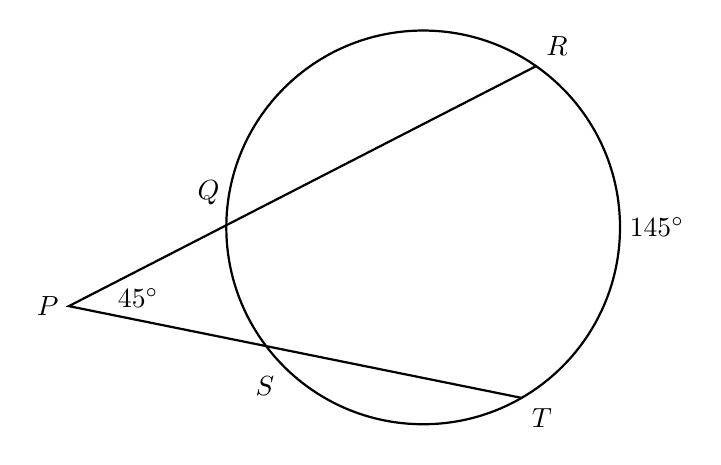
\begin{tikzpicture}[scale=.5]
           \draw [thick] (0,0) circle[radius=5];
           \draw [thick]
           (-60:5) node[below right]{$T$}--
           (-9,-2) node[left]{$P$}--
           (55:5) node[above right]{$R$};
           \draw (225:5) node[below left]{$S$};
           \draw (170:5) node[left] {$Q$};
           \draw (0:5) node[right] {$145^\circ$};
           \draw (-8,-1.8) node[right] {$45^\circ$};
         \end{tikzpicture}
       \end{center} \vspace{1cm}

\newpage
    \item Given $P(7,-4)$ and $Q(4,-1)$, find the length of $\overline{PQ}$. Simplify the radical.\vspace{4cm}

  \item In the diagram below, $\triangle ABC \sim \triangle DEF$, $DE=35$, $AB=2x$, $AC=4x$, and $DF=7x$. Find $x$.
    \begin{center}
      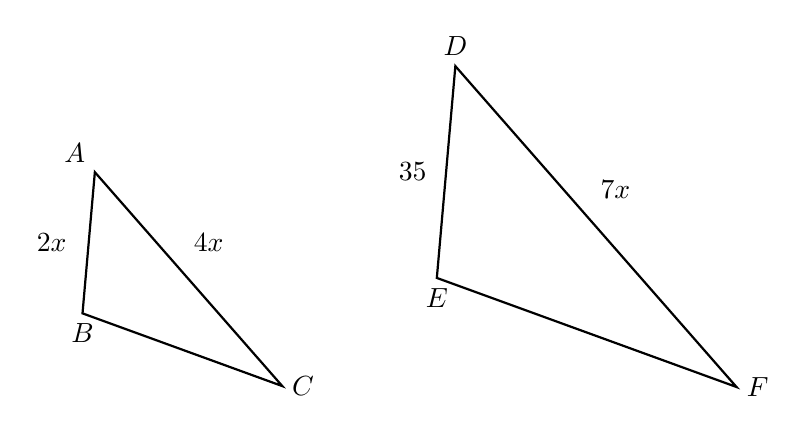
\begin{tikzpicture}[scale=0.9]
      \coordinate [label=above left:$A$](A) at (85:2);
      \coordinate [label=below:$B$](B) at (0, 0);
      \coordinate [label=right:$C$](C) at (-20:3);
        \draw [thick] (A)--(B)--(C)--cycle;
        \node at (95:1)[left]{$2x$};
        \node at (35:1.75)[right]{$4x$};
        \draw [thick, xshift=5cm, yshift=0.5cm] (85:3) node[above]{$D$}--
        (0,0) node[below]{$E$}--
        (-20:4.5) node[right]{$F$}--cycle;
        \draw [thick, xshift=5cm, yshift=0.5cm](90:1.5) node[left]{$35$};
        \draw [thick, xshift=5cm, yshift=0.5cm](30:2.5) node[right]{$7x$};
    \end{tikzpicture}
  \end{center} \vspace{2cm}

   \item In right triangle $ABC$ shown below, point $D$ is on $\overline{AB}$ and point $E$ is on $\overline{BC}$ such that $\overline{AC} \parallel \overline{DE}$. If $AB=20$, $BC=15$, and $AD=8$, what is the length of $\overline{BE}$?
     \begin{center}
       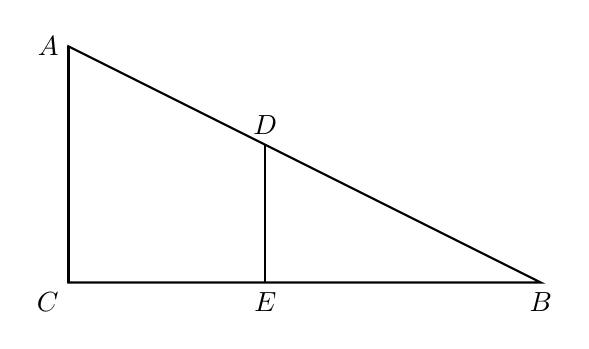
\begin{tikzpicture}[scale=0.5]
         \coordinate [label=left:$A$](A) at (-12,6);
         \coordinate [label=below:$B$](B) at (0, 0);
         \coordinate [label=below left:$C$](C) at (-12,0);
         \coordinate [label=above:$D$](D) at (-7, 3.5);
         \coordinate [label=below:$E$](E) at (-7,0);
         \draw [thick] (A)--(B)--(C)--cycle;
         \draw [thick] (A)--(C);
         \draw [thick] (D)--(E);
       \end{tikzpicture}
     \end{center}

\newpage
  \item What series of transformations map $\triangle ABC$ onto $\triangle DEF$, shown below? Fully specify the transformations.
    \begin{center}
      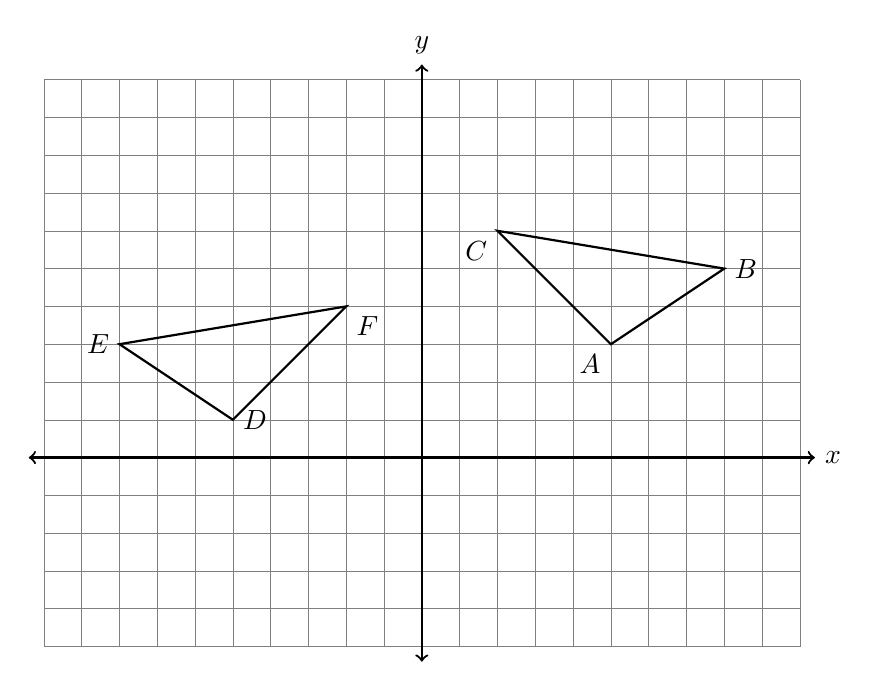
\begin{tikzpicture}[scale=.48]
        \draw [help lines] (-10,-5) grid (10,10);
        \draw [thick, <->] (-10.4,0) -- (10.4,0) node [right] {$x$};
        \draw [thick, <->] (0,-5.4)--(0,10.4) node [above] {$y$};
        \draw [thick]
          (5,3) node[below left] {$A$}--
          (8,5) node[right] {$B$}--
          (2,6) node[below left] {$C$}--cycle;
        \draw [thick]
          (-5,1) node[right] {$D$}--
          (-8,3) node[left] {$E$}--
          (-2,4) node[below right] {$F$}--cycle;
      \end{tikzpicture}
    \end{center}
\vspace{1cm}

 \item Triangle $ABC$ is dilated with a scale factor of $k$ centered at $A$, yielding $\triangle ADE$, as shown. Given $AB=12$, $BC=15$, $AC=18$, and $DE=25$. \\[0.25cm] Find $BD$, $AE$, and $k$ (the scale factor). \vspace{0.5cm}
 \begin{center}
     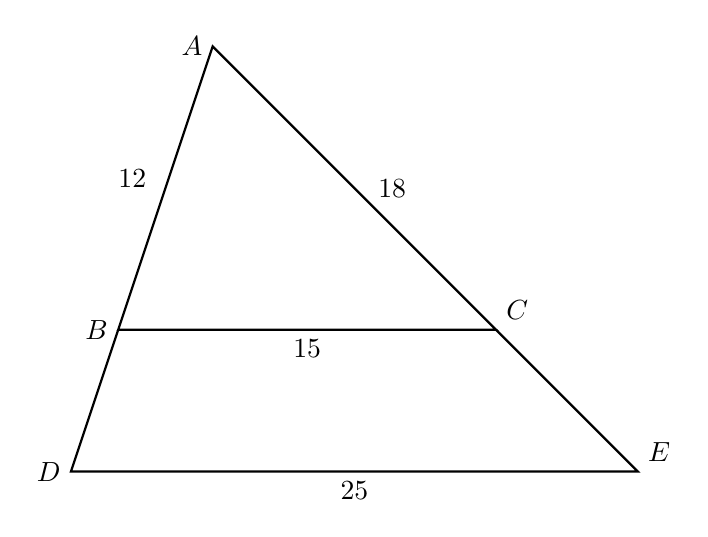
\begin{tikzpicture}[scale=0.6]
       \draw [thick]
       (0,0)node[left]{$B$}--
       (8,0)node[above right]{$C$}--
       (2,6)node[left]{$A$}--cycle;
       \draw [thick]
       (0,0)--
       (-1,-3)node[left]{$D$}--
       (11,-3)node[above right]{$E$}--(8,0);
       \node at (4,0)[below]{$15$};
       \node at (5.3, 3)[right]{$18$};
       \node at (0.3, 2.8)[above]{$12$};
       \node at (5,-3)[below]{$25$};
     \end{tikzpicture}
   \end{center}
\vspace{4cm}

\newpage

  \item What is the length of the segment $A(2,10)$, $B(-4,2)$?
    \vspace{4cm}

  \item What is the equation of a line through the point $A(3,-5)$ and parallel to the line $y=\frac{3}{5}x+1$? (hint: use the point-slope formula, $y-y_A=m (x-x_A)$) \vspace{2.5cm}


  \item The line $l$ has the equation $y=\frac{4}{3}x+3$. To each line below, circle whether $l$ is parallel, perpendicular, or neither.
    \begin{enumerate}
      \item parallel \quad perpendicular \quad neither \qquad $y=\frac{3}{4}x-5$
      \vspace{0.5cm}
      \item parallel \quad perpendicular \quad neither \qquad $y=-\frac{4}{3}x-9$
      \vspace{0.5cm}
      \item parallel \quad perpendicular \quad neither \qquad $3x+4y=-15$
      \vspace{2cm}
      \item parallel \quad perpendicular \quad neither \qquad $4x-3y=6$
      \vspace{1.7cm}
    \end{enumerate}

  \item Simplify each expression. (Leave it in radical form if necessary, not a decimal.)
    \begin{enumerate}
      \begin{multicols}{2}
      \item   $\sqrt{144}$ \vspace{1.25cm}
      \item   $\sqrt{50}$
      \item   $\sqrt{32}$ \vspace{1.25cm}
      \item   $\sqrt{\frac{49}{16}}$
      \end{multicols}
    \end{enumerate}

\newpage

 \item Given $\triangle ABP$ and $\triangle JKP$ as shown below. $\overline{AB} \parallel \overline{JK}$. $AP=6$, $JP=14$, and $JK=21$. Find $AB$.
 \begin{center}
   \begin{tikzpicture}[scale=1.4]
       \draw [thick]
         (0.25,-1)node[right]{$B$}--
         (-0.5,2)node[left]{$K$}--
         (4,0)node[right]{$J$}--
         (0,0)node[above right]{$P$}--
         (-2,0)node[left]{$A$}--cycle;
     \end{tikzpicture}
     \end{center}
 \vspace{2cm}


   \item The grid shows $\triangle ABC$ and $\triangle DEF$.
     \begin{center}
       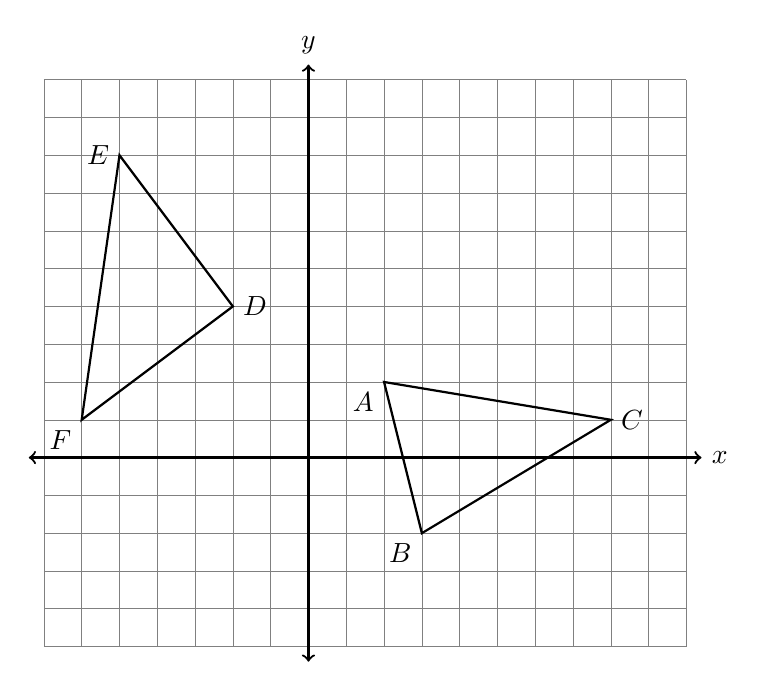
\begin{tikzpicture}[scale=.48]
         \draw [help lines] (-7,-5) grid (10,10);
         \draw [thick, <->] (-7.4,0) -- (10.4,0) node [right] {$x$};
         \draw [thick, <->] (0,-5.4)--(0,10.4) node [above] {$y$};
         \draw [thick]
           (3,-2) node[below left] {$B$}--
           (8,1) node[right] {$C$}--
           (2,2) node[below left] {$A$}--cycle;
         \draw [thick]
           (-2,4) node[right] {$D$}--
           (-5,8) node[left] {$E$}--
           (-6,1) node[below left] {$F$}--cycle;
       \end{tikzpicture}
     \end{center}
     Let $\triangle A'B'C'$ be the image of $\triangle ABC$ after a rotation about point $A$. Determine and state the location of $B'$ if the location of point $C'$ is $(1,-4)$. Explain your answer, supported by stating the transformation applied.

 \newpage

   \item What is the smallest non-zero angle of rotation about its center that would map the pentagon onto itself? \vspace{0.25cm} %$ABCDE$
   \begin{center}
       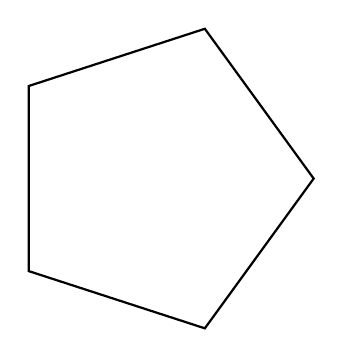
\begin{tikzpicture}%[scale=.48]
         \draw [thick]
         (0:2)--% node[right] {$A$}--
         (72:2)--% node[above right] {$B$}--
         (144:2)--% node[above left] {$C$} --
         (216:2)--% node[left] {$D$}--
         (288:2)--cycle;% node[right] {$E$}--cycle;
       \end{tikzpicture}
     \end{center} \vspace{0.5cm}

  \item Triangle $ADE$ and its midline $\overline{BC}$ are drawn, with $B$ the midpoint of $\overline{AD}$ and $C$ the midpoint of $\overline{AE}$. The two medians $\overline{BE}$ and $\overline{CD}$ are drawn, as shown, intersecting in point $F$, the centroid.\\[0.25cm]
  $\triangle FCB \sim \triangle FDE$ with scale factor $k=2$.\\[0.25cm]
  Given $BC=9$, find $DE$. \\[0.25cm] Given $FE=12$, find $BF$. %\vspace{1cm}
  \begin{center}
      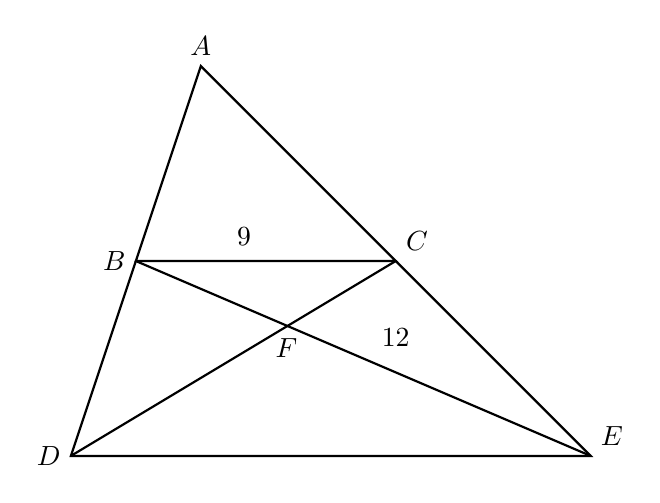
\begin{tikzpicture}[scale=0.55]
        \draw [thick]
        (0.5,1.5)node[left]{$B$}--
        (6.5,1.5)node[above right]{$C$}--
        (2,6)node[above]{$A$}--cycle;
        \draw [thick]
        (0.5,1.5)--
        (-1,-3)node[left]{$D$}--
        (11,-3)node[above right]{$E$}--(6.5,1.5);
        \draw [thick] (0.5,1.5)--(11,-3);
        \draw [thick] (6.5,1.5)--(-1,-3);
        \node at (3,2.5)[below]{$9$};
        \node at (3.5, -0.5)[right]{$F$};
        \node at (6.5, -.7)[above]{$12$};
        %\node at (-0.7, -1)[above]{$5$};
      \end{tikzpicture}
    \end{center} \vspace{1cm}

  \item Write down the center and radius of each circle.
    \begin{enumerate}
      \begin{multicols}{2}
      \item   $(x+1)^2+(y-1)^2=16$ \vspace{2cm}
      \item   $(x-2)^2+(y-7)^2=25$ \vspace{2cm}
      \end{multicols}
    \end{enumerate}

\newpage
 \item Determine and state the transformation or sequence of transformations  applied to $\triangle ABC$, mapping it onto $\triangle PQR$, as shown.
   \begin{center}
       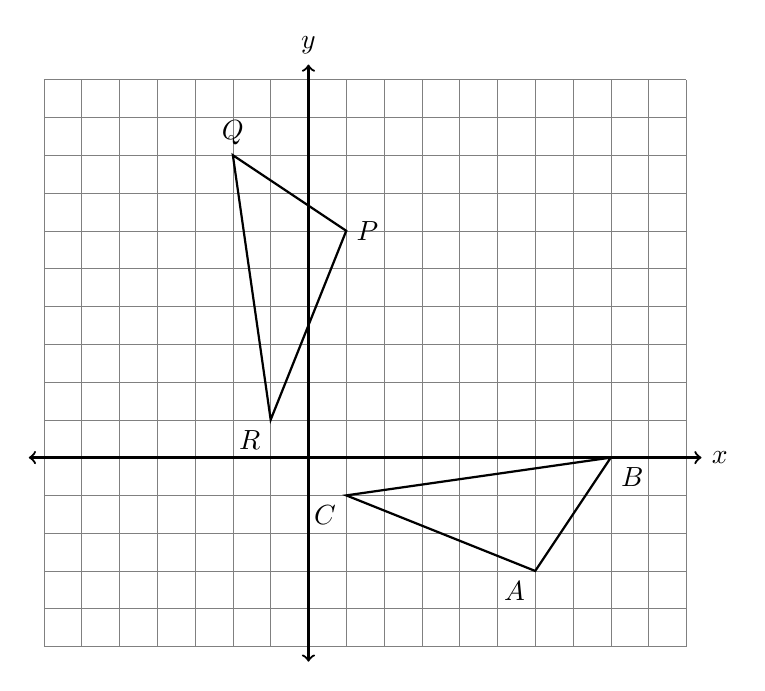
\begin{tikzpicture}[scale=.48]
         \draw [help lines] (-7,-5) grid (10,10);
         \draw [thick, <->] (-7.4,0) -- (10.4,0) node [right] {$x$};
         \draw [thick, <->] (0,-5.4)--(0,10.4) node [above] {$y$};

         \draw [thick]
         (6,-3) node[below left] {$A$}--
         (8,0) node[below right] {$B$}--
         (1,-1) node[below left] {$C$}--cycle;

         \draw [thick]
         (1,6) node[right] {$P$}--
         (-2,8) node[above] {$Q$}--
         (-1,1) node[below left] {$R$}--cycle;
       \end{tikzpicture}
     \end{center}
\vspace{2cm}

  \begin{multicols}{2}[\item The diagram below shows $\triangle ABC$, with $\overline{AEB}$, $\overline{ADC}$, and $\angle ACB \cong \angle AED$. $AB=14$, $AD=8$, and $DE=4$.]
      \begin{enumerate}
        \item $\overline{AE} \rightarrow$ \rule{2cm}{0.15mm} \vspace{0.5cm}
        \item $\overline{AD} \rightarrow$ \rule{2cm}{0.15mm} \vspace{0.5cm}
        \item $\triangle ADE \sim$ \rule{2cm}{0.15mm} \vspace{0.5cm}
        \item What is the scale factor?\\[0.5cm] $k=$  \rule{2cm}{0.15mm}
        \item What is the length of $\overline{BC}$?
      \end{enumerate}
       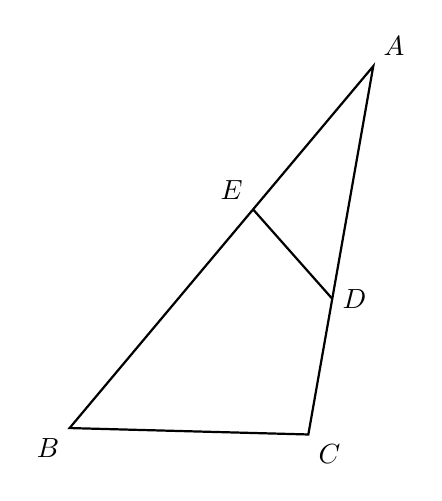
\begin{tikzpicture}%[scale=.48]
         \draw [thick]
         (0,0) node[above right] {$A$}--
         (230:6) node[below left] {$B$}--
         (260:4.75) node[below right] {$C$}--cycle;
         \draw [thick]
         (230:2.375) node[above left] {$E$}--
         (260:3) node[right] {$D$}--cycle;
       \end{tikzpicture}
     \end{multicols}

\newpage


  \item Given $\triangle JKL \sim \triangle MNO$. $m\angle J = 43^\circ$ and $m\angle L = 92^\circ$.\\
  Find the measure of $\angle N$. \vspace{1.5cm}

  \item A translation maps $A(3,5) \rightarrow A'(-2,7)$. What is the image of $B(-4,1)$ under the same translation?  \vspace{1.5cm}


  \item Given $A(-3,5)$ and $B(0,-1)$, find the length of $\overline{AB}$. Leave the result in simplified radical form (not a decimal).

\newpage
\emph{Early finishers}
  \item In the diagram below, the chords $\overline{AE}$ and $\overline{BD}$ intersect at $C$, with $\triangle ABC \sim \triangle DEC$, $BC=3$, $AC=4$, and $AE=11$. Determine the length of $\overline{CD}$.
      \begin{center}
      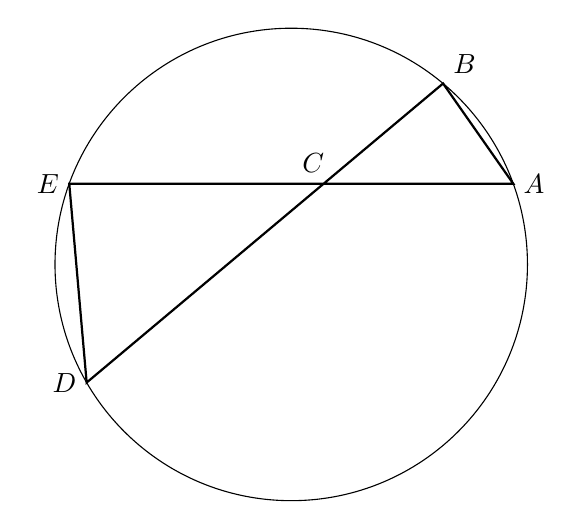
\begin{tikzpicture}[scale=.6]
        \draw (0,0) circle[radius=5];
        \draw [thick]
        (20:5) node[right] {$A$}--
        (160:5) node[left] {$E$}--
        (210:5) node[left] {$D$}--
        (50:5) node[above right] {$B$}--cycle;
        \draw (75:1.8) node[above] {$C$};
      \end{tikzpicture}
    \end{center}

\vspace{2cm}



\end{enumerate}
\end{document}
